\chapter{Main alternatives, Decision and Development of the best one}

\section{Orbits}
\import{sections/OrbitDesign/}{Ch2-OrbitalCoverage}
\import{sections/OrbitDesign/}{Ch3-ConstConfig}
\import{sections/OrbitDesign/}{Ch4-OrbitPerturbations}
\import{sections/OrbitDesign/}{Ch5-Decision}


\section{Space Segment Systems. Satellite Design}
\import{sections/SatelliteDept/}{SatDesign}

\section{Ground Segment Systems}
\import{sections/CommunicationsDept/}{Ch3-GroundSegmentDesign}

\section{Protocol Stack}
\import{sections/CommunicationsDept/}{Ch1-SpaceSegment}
\import{sections/CommunicationsDept/}{Ch2-GroundSegment}

\section{Launcher and Deployer}
\subsection{Launching System}
The aim of this section is the selection of a launching platform. First of all, a review of the available ones on the market is carried out, secondly a small group of launchers is chosen and finally, an optimization is developed in order to find the most suitable system. 

\subsubsection{Launch site and vehicle analysis}
A general research is done in order to filter all the launchers that can be discarded without any study. The result of this research is that there are seven potential rockets in the market capable of deploying the constellation as well as carrying out the replacement needs. The launchers can be divided in two categories: the powerful ones and the small ones. The first ones are capable of carrying heavy payloads, however they present high operation costs whereas the second ones are way more economic due to the reduced size. In addition, the small rockets are more focused on commercial flights without having to attend governmental issues. A table of this seven candidates is shown in the \cite[Chapter 1, Section 1]{annex2}.

Once this first selection is done, more accurate information is needed so as to reach a reliable conclusion. However, none of the enterprises shows its information on the Internet or any similar divulgation channel with the exception of Arianespace. Thus, all of them must be contacted to get the needed data. The same email is sent to all seven enterprises and several days later, three of them show interest in the Astrea constellation: Rocket Labs, PLDSpace and LEO Launch \& Logistics. Since the other enterprises do not answer the requests and, as a consequence, will not provide the necessary information, they can be directly discarded. Hence, the candidates list is reduced to those three who responded the enquire plus Vega, given that its information is available online. 

In order to find the most suitable option achieving the project objectives, it is thought to do an evaluation process following the Ordered Weighted Average (OWA) method . First of all, the required parameters for the decision have to be determined. According to the orbit design, the range of inclinations, the number of orbital planes and the range of heights must be taken into an account. Nevertheless, more parameters are needed in order to ensure a reliable result: cost per satellite, frequency of launchings per year and number of satellites deployed per launch. Both range of inclinations and number of satellites per launch act as a restriction due to the following two reasons. First, since orbital plane changes are very expensive and are out of consideration, the minimum number of launchings must equal the number of orbital planes. In addition, being capable of deploying the constellation with the minimum number of launchings is an adequate solution. This turns the number of CubeSats per launch into a restriction: the chosen launcher must be capable of launching at least the number of satellites in an orbital plane. Secondly, the inclination is considered a restriction by the fact that if a rocket is not capable of deploying a satellite in the desired inclination, it makes no sense to use it. 

Since the number of orbital planes is 8 and the inclination is 72$^{\circ}$, any launcher which doesn't fulfills one of this restrictions can be automatically rejected. 

Moreover, the following table contains all the information mentioned above which is helpful to compare the different launchers and see if they accomplish the basic features. 

\begin{table}[h]
\begin{center}
\begin{tabular}{|c|c|c|c|c|}
\hline
\bf{Parameters} & \bf{Rocket Lab} & \bf{PLD} & \bf{LEO L\&L} & \bf{Vega}\\
\hline 
\bf{Satellites/Launch} & 24 & 34 & 150 & 325 \\
\hline 
\bf{Inclination($^{\circ}$) } & {39.2 to 99} & {116 or 140} & {any} & {any}\\
\hline 
\bf{Cost/Satellite (US dollars)} & 240,000 & - & 266,667 & 100,000\\
\hline 
\bf{Orbital planes} & 1 & 1 & 1 & 1 \\
\hline 
\bf{Frequency/year} & 9 & 8 & 8 & 2 \\
\hline 
\bf{Range of heights (km)} & LEO & LEO & LEO & LEO\\
\hline
\end{tabular}
\end{center}
\caption{Criteria}
\end{table} 

It is important to point out that all the rockets available in the market can achieve the necessary amount of satellites per launch. Although all of them reach the height the CubeSats need, PLD does not attempt the inclination needed which is 72$^{\circ}$. As a result, this launcher is not appropriate for the project purpose and it is rejected. 

According to the remaining 3 candidates, all of them are adequate candidates, nevertheless there is a characteristic that may interfere with the mission goals. At first instance, the frequency per year has not been considered a critical parameter. Those have been chosen regarding orbital parameters only, however, although the frequency does not influence de capability of the rocket of deploying a CubeSat in the desired orbit, it can compromise the set up of the constellation and the posterior replacements. The lower the frequency is, the slower the deployment will be. Therefore, the frequency of the three remaining candidates must be analyzed. As seen in the table, Vega presents the lowest frequency (two launchings per year). This value is not acceptable due to the intention of deploying one single orbital plane per launch. The placement of the whole constellation would last four years, this mean that de first planes would be near their replacement time while the last ones would only have been nearly a year in orbit. Thus, Vega can also be discarded.
 
This leaves the selection with only two options: Rocket Lab and LEO Launch\&Logistics. An Ordered Weighted Average can be made between those two candidates taking the cost/satellite, the number of orbital planes, the frequency and the range of heights into account. Yet, they both present the same number of planes and range of heights, consequently the OWA can be done regarding only the two cost and frequency. The first has to be minimized and the second maximized. Since Rocket Lab presents best values in one parameter and the other (240,000 US dollars vs 266,667 and 9 launchings/year vs 8) there is no need to develop an OWA. In addition, an e-mail from Rocket Lab is received stating that a launch per week is achievable. Thus, the chosen rocket is Electron, from Rocket Lab enterprise. This rocket fulfills all the requirements of the constellation. 

As it is given in Rocket Lab payload users guide \cite{Guide2016}, Electron is a two stage light rocket constructed from carbon fiber composite. It is powered by ten Rutherford engines, all of them use liquid oxygen (LOX) and rocket kerosene. The first stage has nine out of the ten engines which generate 152 kN of thrust. The second one, has the remaining engine which produces 22 kN. The second stage contains the fairing where the payload is placed. Electron is 17 m long and its diameter is 1.2 m. It is capable of launching 24 3U CubeSats every week at a LEO orbit with a range of inclinations from 39.2 to 99 degrees. 

Rocket Lab facilities are located in New Zeland. The test laboratories are placed near the airport of Auckland and the launch site is in Mahia.

Finally, the cost per satellite is 240.000 US dollars or if the rocket is totally filled, 5.760.000 US dollars the entire launch. Some images of Electron are showed in the  \cite[Chapter 1, Section 1]{annex2}, a picture of the launching site is also showed.  %  Section 2: Launching System
\subsection{Deployer}
The objective of this section is to give a brief explanation of what is a deployer and how it works. 
As introduced above, there must be an adaptor between the rocket and the satellite in order to ensure subjection during the flight, efficient organization of the space in the fairing and a correct separation during the injection maneuver. This duty falls on the deployer. It consists on a prismatic structure prepared to carry the CubeSat inside. When the desired orbit is reached, the deployer uncovers one of its faces so as to let the satellite leave. There is a spring in the bottom that provides a little push to ensure that the CubeSat separates from the rocket.

There are many types of deployers, some of them are designed for an specific type of mission. As stated before, Electron is compatible with the standard CubeSat deployers, hence, only this type is considered. Similar to the case of the launcher selection, almost all the enterprises don't show enough information on the internet to reach a reliable conclusion, thus, some of them are contacted. Only two answers are obtained, one from ISIS (ISIPOD Deployer) and GAUSS (GPOD deployer). POD stands for Pico-satellite Orbital Deployer. 

They both present similar characteristics, however there are some differences. The main characteristics of the two deployers are listed in the ANNEX, also two pictures of them are shown there.

In order to reach a reliable conclusion, two issues must be taken into consideration. First, the CubeSats of the Astrea Constellation are equipped with thrusters which increase the length of the satellite, thus, the deployer chosen cannot be fully closed. As seen in the ANNEX, GPOD has accessible panels whereas ISIPOD is fully closed, hence, ISIPOD is not suitable for the needs of the Astrea constellation. This condition automatically rejects the ISIPOD, nevertheless, there is a second reason for choosing the GPOD, the enterprise ISIS does not show the prices of their deployers even when a request is sent. Without this information it is decided that it cannot be taken into account. The price for the GPOD  deployer is 16000 US dollars per unit.  % Section 3: Deployer

\section{Lifecycle Strategies}
%%%%%%%%%%%%%%%%%%%%
% - - - - - - - - PART JOAN - - - - - - - - - 
%%%%%%%%%%%%%%%%%%%%
\section{First Placement}
The aim of this part is to explain the first placement of the constellation. It is divided in two parts. The first one is intended to give a first approach to the logistics involved in the first placement, whereas the second one is focused on the maneuver required so as to deploy the satellites into orbit. 

\subsection{First Placement logistics}
Gantt charts provided by Rocketlab USA:

\begin{figure}[H]
\centering 
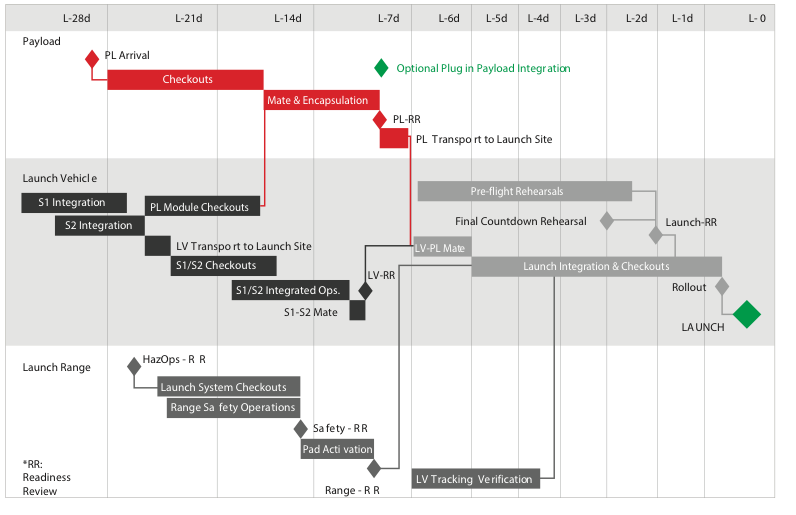
\includegraphics[scale=0.7]{./sections/Constellation_Deployment/S4-First_Placement/Images_S4/Picture_1_S4.png} 
\caption{Launch Range Operations Flow/Schedule}
\label{fig:gantt1}
\end{figure}

\begin{figure}[H]
\centering 
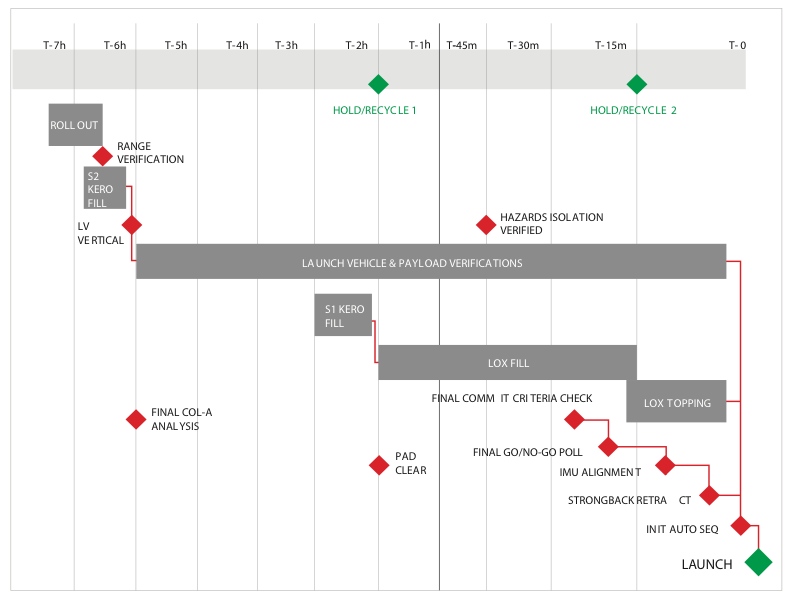
\includegraphics[scale=0.7]{./sections/Constellation_Deployment/S4-First_Placement/Images_S4/Picture_2_S4.png} 
\caption{Countdown Operations Flow}
\label{fig:gantt2}
\end{figure}

%%%%%%%%%%%%%%%%%%%%%%%%%%%%%%%%%%%%%%%%
% - - - - - - - - - PART ROGER - - - - - - - - - - 
%%%%%%%%%%%%%%%%%%%%%%%%%%%%%%%%%%%%%%%%
\subsection{1st Placement In-Orbit Injection Maneuver}
In a more schematic way, the procedure goes as follows:

\begin{enumerate}
\item The rocket goes through the procedure designed by Rocketlab USA to get to the destination orbit. The approximate trajectory during this stage is represented in \ref{orbit1}.Right after entering into the destination orbit, the first satellite is deployed into it as seen in \ref{orbit1} represented with a red dot.
\item Once the latter is completed, the rocket's engine gives it the necessary $\Delta V$ in order to get to the elliptical spacing orbit. In \ref{orbit2} half a revolution of the rocket is represented along with the orbit of the first deployed satellite at the same point in time.
\item After one full revolution of the rocket in the elliptical orbit, the first satellite will have left the right phase spacing with respect to the rocket. At this point the rocket's engine gives the same $\Delta V$ as in step 2 but negative. This will cause it to enter again into the circular orbit of the satellites. At this point the rocket deploys the second satellite as shown in \ref{orbit3}. Right after this deployment the rocket enters into the elliptical orbit again.
\item \ref{orbit4} represents again half a revolution of the rocket in the elliptical orbit along with the deployed satellites so far.
\item Finally, the rocket reduces its velocity again to enter into the circular destination orbit in order to deploy the third satellite (\ref{orbit5}).
\item This aforementioned procedure is iterated until the orbital plane is full.
\newline\newline
\end{enumerate}

\begin{figure}[H]
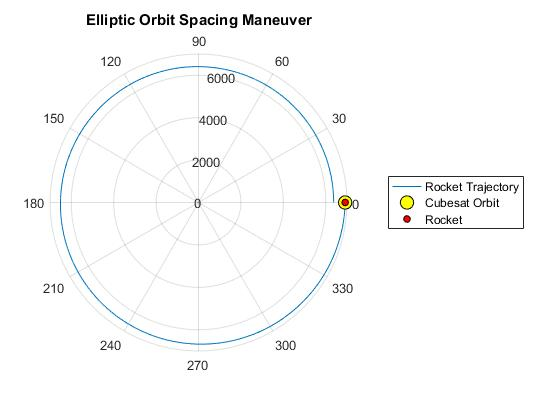
\includegraphics[scale=0.7]{./sections/Constellation_Deployment/S4-First_Placement/Images_S4/Picture_3_S4.jpg}
\caption{Rocket's trajectory from lift-off to final orbit.}
\label{orbit1}
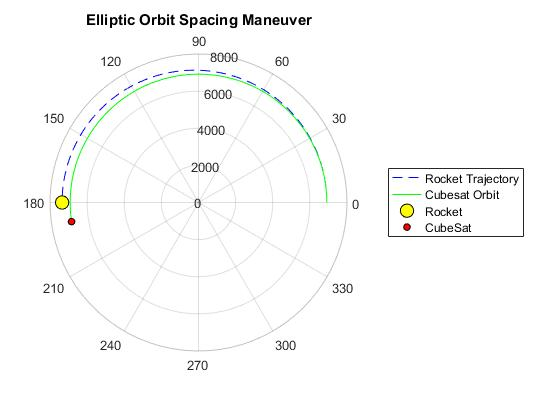
\includegraphics[scale=0.7]{./sections/Constellation_Deployment/S4-First_Placement/Images_S4/Picture_4_S4.jpg}
\caption{Half of a revolution of the rocket in the elliptical spacing orbit.}
\label{orbit2}
\end{figure}

\begin{figure}[H]
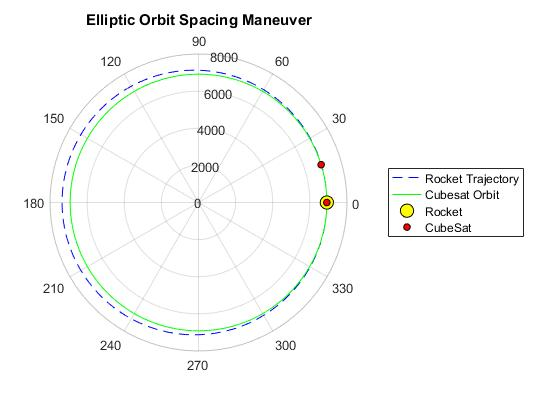
\includegraphics[scale=0.7]{./sections/Constellation_Deployment/S4-First_Placement/Images_S4/Picture_5_S4.jpg}
\caption{Deployment of the second satellite.}
\label{orbit3}
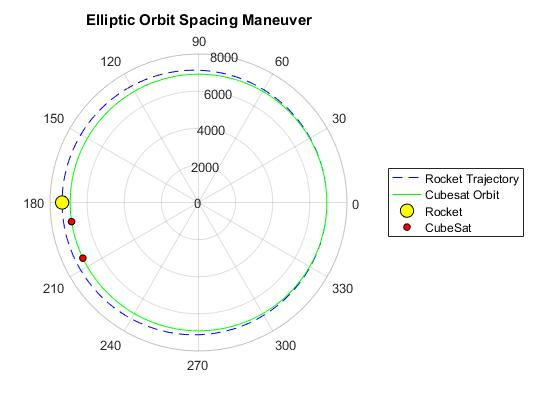
\includegraphics[scale=0.7]{./sections/Constellation_Deployment/S4-First_Placement/Images_S4/Picture_6_S4.jpg}
\caption{Half of a revolution of the rocket after the deployment of the second satellite.}
\label{orbit4}
\end{figure}

\begin{figure}[H]
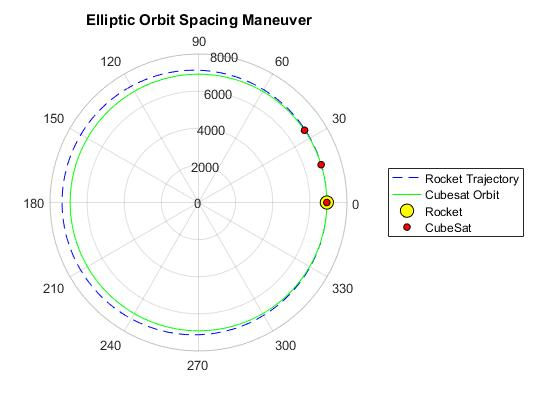
\includegraphics[scale=0.7]{./sections/Constellation_Deployment/S4-First_Placement/Images_S4/Picture_7_S4.jpg}
\caption{Deployment of the third satellite.}
\label{orbit5}
\end{figure}

\subsection{Orbit Parameters Calculation}
\begin{center}
$V_s = \sqrt{\frac{GM_t}{R_t\,+\,h}} $
\newline\newline
$T_s = \frac{2\pi(R_t\,+\,h)}{V_s}$\newline
\end{center}

Where $R_t$ and h are Earth's radius and height above Earth's surface respectively. For $h = 542 \,km$, the values obtained are $V_s = 7,589.6 \,m/s$ and $T_s = 5,723.1 \,s$. Let's call the spacing between satellites $\theta = \frac{360^\circ}{21} = 17.14^\circ$ and $R = R_t \,+ \,h$. Using these values it is possible to compute the period of the elliptical orbit, $T_r$, along with the rest of the parameters:

\begin{center}
$T_r = T_s\,+\,\frac{\theta R}{V_s} = 5,995.6\,s$

$a = (\frac{T_r}{2\pi}^2GM_t)^\frac{1}{3}=7,130.8\,km$

$R_1 = R;\;\;\;R_2=2a\,-\,R_1$

$c = a\,-\,R_1;\;\;\;b = \sqrt{a^2\,-c^2}$

$\epsilon = \sqrt{1\,-\,\frac{b^2}{a^2}}=0.0305$

$\Delta V = \sqrt{\frac{GM_t}{R1}}\,(\sqrt{\frac{2R_2}{R1\,+\,R2}}-1)=115.01\,m/s$

\end{center}

\subsubsection{Plane Order}
The aim of this section is to describe the order in which all of the 9 planes are put into orbit. The fact that establishes one path or another is the fact that satellites can only communicate with neighbours, that is, one satellite can only communicate with its neighbours from the same plane and the neighbours from the neighbour planes.

When it comes to the order in which the planes are put into orbit, there are two main ways that come to mind. The first one is putting the planes consecutively into orbit. The second one is to put the planes into orbit leaving space between them for future planes. For example plane number one is put into orbit. The second plane to be put into orbit leaves space for one plane in between them. Then the third leaves space for one plane from the second, and so on. Leaving more space than for one plane could also be an option.

On the one hand, when using the first way the satellites from each plane could communicate with the ones from their neighbourhood. Therefore the range of communication would start being narrower but as new planes are put into orbit, the range would become wider. For instance, when three planes are already working, a given satellite form a customer could communicate with satellites that are at the other side of the planet in a determined range given by the width of signal that those three orbital planes could cover. When new planes are put into orbit this width becomes bigger up until the full globe is covered. Of course the main drawback of using this consecutive way of putting planes into orbit would be the long time of inactivity right at the beginning when few planes are working.

On the other hand, when using the second described way, the satellites can't communicate with other satellites from neighbour planes but the time of inactivity for customer's satellites would be less as a gap between planes is left for future ones. Nevertheless, this kind of configuration has a huge drawback and it's that when a satellite communicates with one given plane, this one can only communicate with other satellites that are in the range of signal emission of that given plane. This is due to the fact that as neighbour planes are further apart they can't communicate with each other and therefore the range of communication is affected.

Having pointed out all of the advantages and drawbacks of each configuration it is time to choose and it all comes down to Astrea's preferences. The configuration that fulfills these preferences for the most part is the consecutive one. It allows the satellites to communicate in a broader range as the constellation grows and progressively conquer the sky. % Section 4: First Placement
\subsection{Replacement Strategy}
Due to the lifespan of the CubeSats, the whole constellation is replaced every five years, hence, a replacement strategy has to be designed. As stated in the First Placement section, the orbital planes are deployed consecutively, thus, the replacement has to be so also. One simple solution could be waiting for a plane to de-orbit and then place a new one into the same position, however, this procedure would spend to much time by the fact that the satellites approach the atmosphere in a very slow rate. Additionally, the replacement of different planes would probably overlap. Since the first placement has been carefully designed, it is thought to adapt the same procedure to the replacement process, that means, to consider the replacements as a first placement. Obviously, some differences have to be taken into account given that at this point there is a constellation providing full service to the customers. The problem remains on the fact that in order to use the same strategy, the replacement needs to be achieved in eight weeks, therefore, the new orbital planes cannot be situated into the same position than the old ones. A rapid replacement is also interesting regarding the need of providing full service to the customers without interruption. The solution adopted consists on placing the new planes between the old ones consecutively, following the order of the first placement. In order to clarify the process, a detailed explanation is shown below:
\newline\newline
First of all, since different orbital planes are going to be taken into account in this explanation a nomenclature is set: old planes are the ones that have to be replaced, the new ones are the planes that will substitute them. If a plane is named with the number 1, it means that is the first one to be placed (old or new) and so on (2,3,..,21). 
\begin{itemize}
\item The new plane 1 is placed between the old plane 1 and the old plane 21.
\item The new plane 2 is placed between the old plane 1 and the old plane 2 to ensure that at the very moment the first old plane begins to decay, it does not appear a gap.
\item At this point, the following new planes are deployed consecutively between the old ones until the constellation is fully renovated. This maneuver is repeated every five years to ensure the continuity of the Astrea Constellation. 
The following images show the process explained above.
\end{itemize}
\begin{figure}[h!]
\centering 
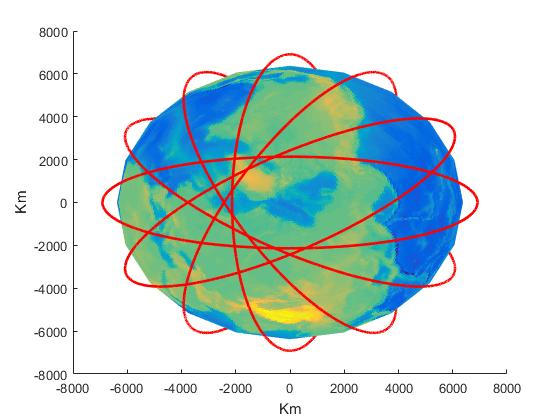
\includegraphics[scale=0.7]{./sections/Constellation_Deployment/S5-1-Replacement_Strategy/Images_S5-1/Picture_1_S5-1.jpg} 
\caption{Old Constellation}
\label{fig:rp1}
\end{figure}

\begin{figure}[h!]
\centering 
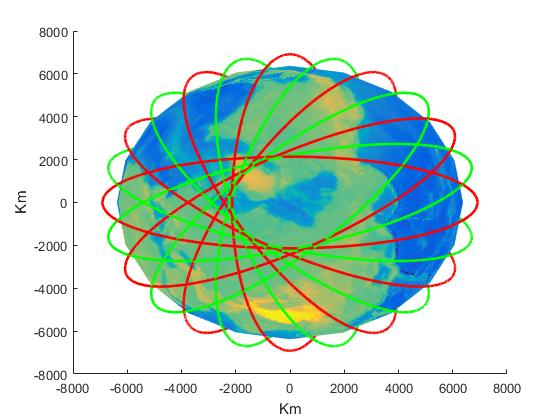
\includegraphics[scale=0.7]{./sections/Constellation_Deployment/S5-1-Replacement_Strategy/Images_S5-1/Picture_2_S5-1.jpg} 
\caption{Old and New Constellations}
\label{fig:rp2}
\end{figure}

\begin{figure}[h!]
\centering 
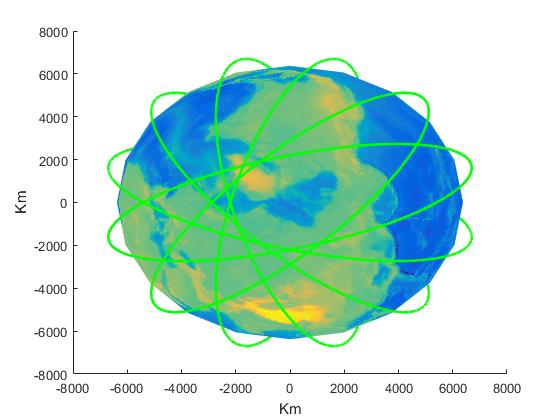
\includegraphics[scale=0.7]{./sections/Constellation_Deployment/S5-1-Replacement_Strategy/Images_S5-1/Picture_3_S5-1.jpg} 
\caption{New Constellation}
\label{fig:rp3}
\end{figure}

 % Section 5-1: Replacement Strategy
\section{Spare Strategy}
\subsection{Introduction}
When building a satellite constellation with the target to provide global coverage communication relay between LEO satellites and between LEO satellites and the ground, it is crucial to avoid any deterioration of the service. In order to ensure that any possible fail from the satellites would not spoil the constellation operation for more than 6 hours; a spare strategy has to be done. Nowadays, four different types of spare strategies are known:
\begin{itemize} 

\item {Spare satellites in constellation}
\item {In-orbit spare} 
\item {Spare satellites in parking orbits} 
\item {Spare satellites on the ground} 

\end{itemize}
Each existing spare strategy is valid. Despite, depending on the enterprise prioprities the most suitable has to be choosen. In addition, the decision taken is related to the constellation flexibility to degrade the service to a lower performance level during a certain period and to its cost. 

\subsection{Spare Strategy Alternatives}

\textbf{Spare satellites in constellation:}
\newline
This configuration consists on designing the constellation to be \textit{ "overpopulated"}. As it sounds, this means that the system is established with \textit{extra} operative satellites already orbiting within the constellation. For instance, only two overpopulating configurations had been pictured: ovepopulated by one satellite or overpopulated by two satellites per orbital plane. 

\begin{itemize}
\item[-] \textsc{One extra Satellite:}
\newline
By adding an extra satellite to the primary design of the orbital plane configuration, one satellite failure is covered with little time delay to recover the plan. In this way, the constellation continues to work at maximum capacity after a short interruption and at a suitable cost. 
\item[-] \textsc{Two extra Satellites:}
\newline
Usually, by adding two extra satellites per orbital plane the reliability of the service achieves values around the 99.99\%. This configuration increases considerably the cost of the project and it is mainly neccessary in cases where the availability of the satellite is essential for the proper operation of the constellation.
\end{itemize}
Therefore, when designing an overpopulated constallation, the first decition to be made is the number of extra satellite per orbital plane. To guarantee the most optimal configutation a feasibility study is needed.  
\newline
\newline
\textbf{In-orbit spare:}
\newline
The main diference between this strategy and the previous one is that in this case spare satellites are not operative. So the idea is to put some spare satellites in a orbit close to the principal one of the constellation in order to avoid possible collisions between operative satellites and spares. 
\newline
\newline
A few things have to be taken into account when using this method. Firstly,even though the spare satellites are not operative, by being in orbit they deteriorate and by the time they are needed their operative lifetime and performability will not be such as the ones of brand new satellites.Secondly, as their are non-controlled satellites their orbital decay has to be predicted to be aware of possible collitions and avoid them. Thirdly, once any spare satellites is needed, it has to be able to do a two Hohmann transfer to achieve the performance orbit; the first one to reach a phasing orbit and the second one to end in the operational altitude.
\newline
\newline
\textbf{Spare satellites in parking orbits:}
\newline
By mading this choice it has to be assumed that the spare satellites can be keeped in parking orbit until they are needed. Two different option are valid: keeping the rocket in a \textit{"parking"} orbit and then try to send it to the corresponding orbit; or keeping it in in-orbit satellites parkings such as the ISS. The main drawback is that the performance takes a long time until the constellation is recovered and depending on the orbit parameters and the launcher it is not possible to use this strategy.  
\newline
\newline
\textbf{Spare satellites in parking orbits:}
\newline
The simpliest and easiest one; the only thing that has to be done is to build extra satellites. The spares will remain on ground when the constellation is launched. Only in case the structure collapses due to a satellites failure, an emergency launch will put the spares in orbit. Moreover, this method is expensive because every extra launch has a high cost and it can take weeks to recover the constellation performance. 
\newline
\subsection{Spare Strategy Selection}
From all those alternatives, two of them  are quickly discarded: in-orbit spares and in parking orbit spares. The first one is having a non-working satellite in orbit because not only the satellite has to be purchased, but also it has to be launched to a different orbit than the principal one. That fact will increase the cost of the launch or even worst it could create the necessity of an extra launch. Although, the satellites needs to reach the operative orbit and it is known that cubesats propulsion is not really powerful. Furthermore, this satellites might never be needed. So it is highly probable this investment to be a waist of money and sources and this are the main reasons why it has benn discarded.
\newline
\newline
The second is not available in the \textit{Astrea Constellation} case. On the one hand, the main parking in orbit will be the ISS which is at an altitude of 400km above the earth and the constellation is situated at among 550km above the earth. Knowing that, this option is immediately discarded. On the other hand, the Electron the rocket that will accomplish the mission to put the satellites in orbit cannot stay in parking orbit before arriving to its final destination. Definitely, the service cannot rely on this option.
\newline
\newline
Two possible spare strategies remain: pare satellites in the constellation or on ground. In spite deciding if both ones are useful or only one of them is, a feasibility study is done. The objective is analise the diferent kind of failure that have to be covered and determine how the constellation will collapse. Only after that the most suitable strategy method can be designed having as reference the alternatives presented above. 
\subsubsection{Feasibility Studies}
The following studies are based on the probability of failure of the satellites and how the different combinations of failure could become a critical or not for the constellation operations. Furthermore, the main parameters needed during this studies are the number of satellites per plane, the probability of failure of a single satellite and the number of planes. 
\newline
\newline
Let's quantify the parameters presented above. The probability of failure of the satellite during the first five years is about \textbf{FALLABILITAT} and there are 21 satellites per orbital plane per 8 orbital planes. As a result, it means the whole constellations contains 168 satellites which have a 95\% of probability not to fail. By doing quick calculations, firstly it could be assumed that around 8 satellites would fail during the mission. However, this are simple calculations with low reliability.
\newline
\newline
As CubeSat communicate between other satellites and ground, two different cases of failure are observed. On the one hand, the constellation has been designed to offer global coverage of the Earth's surface, so once a satellites fail its footprint disappear and a small hole appears. On the other hand, a sophisticated network of communication between satellites has been created, so once a Cubesat fails it creates a hole in the communications network and entails the creation of new paths which avoid the non-operative satellite. Therefore, the collapse situation for each state has to be determined.
\newline
\begin{itemize}
\item \textsc{Communication with ground:}
The main problem with ground communications is the appearance of a big gap in the footprint the satellites leave. This gap is formed by the failure of several neighboring satellites and has to be big enough to cut all communication with the corresponding ground station to consider the failure as critical. Nevertheless, even if the communication with a single ground station was not possible for a short period of time the information could be transmitted to another ground station with the only drawback that the travel time of the data increases.   
\item \textsc{Communication between satellites:}
Once the communication of a satellite fails, it creates a gap in the communication network. Although any satellite outside the constellation (referring to the ones that use \textit{Astrea} services) tries to communicate, it will not have any problem to communicate with neighboring CubeSat to the one it failed if it is necessary. So the real problem could appear when two or more neighboring CubeSats fail. Additionally, the failure of a single satellite is not critical at all for the constellation because the data can still travel through other paths. 

\end{itemize}

  % Section 5: Spare Strategy
\subsection{Space Debris}
The Space had been a virgin environment until the middle of the twentieth century. However, it has already been exploited by humanity. During the last sixty years many space research centers –such as NASA, ESA or ROSCOSMOS- have been sending rockets and satellites to explore and understand its foreign environment without thinking on the consequences it could have. Fortunately, at the twenty-first century the concern about space debris has appears. Due to this fact, all those space research centers have begun to develop end-of-life strategies for all the missions that generate debris to restrict its lifetime. 

The term space debris implicates all man-made objects that are orbiting with no human control. The problem arises from the fact that depending on the orbital parameters this space stuff is subject to more or less perturbations from either the Earth, the Moon, the Sun or the atmospherically drag and, after their operability’s death, they might never disappear or completely disintegrate. As the quantity of space debris is huge and varied, they have been classified in four categories: fragmentation debris, non-functional spacecraft, rocket bodies and mission related debris. 

\begin{figure}[H]
\centering 
\includegraphics[scale=0.1]{./sections/Constellation_Deployment/S6-End_Of_Life/Images_S6/Picture_1_S6.jpg} 
\caption{View of the Space Debris around the Earth}
\end{figure}

The category that concerns the project is the non-functional spacecraft because it refers to all intact structures which have completed their mission. It is noticed that once satellite’s operative lifetime arrives to its end, the satellites stop maneuvering and counteracting perturbations to maintain the current orbit. Consequently, they tend to deviate from their nominal orbital parameters, starting an unknown trajectory and important repercussions. 

Therefore, by increasing the number of uncontrolled \textit{``dead''} satellites the probability of collision between working satellites and space debris increases at LEO as it is overcrowded. Space debris is small usually and its location can be followed from earth but is impossible to control it. Meanwhile, it is essential for space assets to be free of any impact because avoidance maneuvers are too complicated to have real success.  Thereby, the increasing risk of collision becomes the big threat everyone is fighting against. 

\subsection{End-of-Life Types and Analysis}
As it has been found in \cite{cornara}, End-of-life strategies were implemented taking into account three factors: the time the satellite can orbit, the technical feasibility of active de-orbiting in terms of propellant and sub-systems enhancements, and the altitude of its nominal orbital plane. 

The first one is related to the fact that the current recommendations say that any space asset that can become a non-functional spacecraft must de-orbit and disintegrate at its twenty-fifth birth on orbit. The second refers to the magnitude of the maneuver that can be developed with the power the thruster system can achieve. The third one is relevant because perturbations in space change according to the distance to the Earth’s surface. The closer it is, the more perturbations from Earth and drag forces from the atmosphere the satellite suffers, and perturbations help to de-orbit and disintegrate space assets.

Based on these premises, two different end-of-life groups had been determined: 

\begin{itemize}

\item[-] \textsc{Controlled de-orbit:}

It consists on carrying out a maneuver that leads to a steep, controlled re-entry and burn-up in the atmosphere or ground impact. It must be done in a relatively short period of time, usually 1 revolution and it involves significantly high $\Delta V$. This sophisticated maneuver is initiated by a large increment of potential energy to make change the orbital altitude to a lower one well into the atmosphere where the satellite burns. A few calculations are useful to have a numerical result of that  $\Delta V$:
The velocity in the initial orbit is: 

\begin{center}
$V1 = \sqrt{\frac{GM_t}{R_t\,+\,h}}  = 7593.4 m/s$
\end{center}

Then the semi major axis of the elliptical orbit is obtained: 
\begin{center}
$a = {\frac{r_1+r_2}{2}} = 6672 km$
\end{center}

The speed at apogee of the elliptical orbit is: 

\begin{center}
$V2 = \sqrt{GM_t(\frac{2}{r}-\frac{1}{a})} = 7455 m/s$
\end{center}

Finally, the $\Delta V$ is computed: 
\begin{center}
$\Delta V = V1-V2 = 138.4 m/s$
\end{center}

\item[-]  \textsc{Uncontrolled de-orbit:}

A simpler and cheaper way to de-orbit satellites is to induce a reduction of the orbit altitude in order to cause a decay and, finally, a re-entry to the atmosphere. The process is initiated by one or several arc maneuvers at apogee passes and it is carried out without controlling the trajectory. This procedure is appropriate for low-thrust systems and small satellites. 

In addition, when considering satellites placed at LEOs, this strategy takes advantages of the perturbations present in this altitudes (atmospheric drag). This force contributes to the decay increasing the rate of approach to the atmosphere. 

\end{itemize} % Section 6: End Of Life













